\documentclass[11pt,a4paper]{article}

% Packages
\usepackage[utf8]{inputenc}
\usepackage[english]{babel}
\usepackage{amsmath}
\usepackage{amssymb}
\usepackage{amsthm}
\usepackage{graphicx}
\usepackage{tikz}
\usepackage{algorithm}
\usepackage{algpseudocode}
\usepackage{booktabs}
\usepackage{geometry}
\usepackage{hyperref}
\usepackage{caption}
\usepackage{subcaption}

% TikZ libraries
\usetikzlibrary{shapes.geometric, arrows, positioning, calc}

% Geometry
\geometry{margin=1in}

% Title
\title{\textbf{Market Liquidity Measurement Framework} \\
\large A Comprehensive Model for Trading Book Analysis}
\author{Technical Documentation}
\date{\today}

% Custom commands
\newcommand{\R}{\mathbb{R}}
\newtheorem{definition}{Definition}

\begin{document}

\maketitle

\begin{abstract}
This document provides a comprehensive technical description of a market liquidity measurement framework for analyzing trading positions. The framework incorporates multiple established liquidity metrics including bid-ask spreads, the Amihud illiquidity ratio, volume-based measures, and market impact estimation. We present the mathematical formulations, implementation algorithms, and practical applications of this multi-dimensional approach to liquidity analysis.
\end{abstract}

\tableofcontents
\newpage

\section{Introduction}

Market liquidity represents the ease with which an asset can be bought or sold without causing significant price movement. For portfolio managers and risk managers, understanding the liquidity profile of a trading book is crucial for:

\begin{itemize}
    \item \textbf{Risk Management:} Illiquid positions increase exit costs during market stress
    \item \textbf{Capital Allocation:} Liquidity costs affect expected returns
    \item \textbf{Regulatory Compliance:} Basel III and other frameworks require liquidity assessment
    \item \textbf{Portfolio Optimization:} Liquidity constraints affect optimal portfolio construction
\end{itemize}

This framework provides a systematic approach to quantifying liquidity across multiple dimensions.

\section{Mathematical Framework}

\subsection{Position Representation}

Let a trading position $i$ be characterized by the tuple:

\begin{equation}
P_i = (S_i, Q_i, M_i, B_i, A_i, V_i)
\end{equation}

where:
\begin{align*}
S_i &: \text{Security symbol/identifier} \\
Q_i &: \text{Quantity held (positive for long, negative for short)} \\
M_i &: \text{Current market price (mid-price)} \\
B_i &: \text{Best bid price} \\
A_i &: \text{Best ask price} \\
V_i &: \text{Average daily trading volume}
\end{align*}

The position value is defined as:
\begin{equation}
\text{PV}_i = |Q_i| \times M_i
\end{equation}

\subsection{Bid-Ask Spread Measures}

The bid-ask spread is the most fundamental liquidity measure, representing the immediate cost of a round-trip transaction.

\subsubsection{Absolute Spread}

\begin{equation}
\text{Spread}_{\text{abs},i} = A_i - B_i
\end{equation}

\subsubsection{Relative Spread}

The relative spread normalizes the absolute spread by the mid-price:

\begin{equation}
\text{Spread}_{\text{rel},i} = \frac{A_i - B_i}{\frac{A_i + B_i}{2}} = \frac{A_i - B_i}{M_i}
\end{equation}

This is typically expressed as a percentage.

\subsubsection{Spread in Basis Points}

\begin{equation}
\text{Spread}_{\text{bps},i} = \text{Spread}_{\text{rel},i} \times 10,000
\end{equation}

\subsection{Amihud Illiquidity Ratio}

The Amihud (2002) illiquidity measure captures the price impact per unit of trading volume:

\begin{equation}
\text{ILLIQ}_i = \frac{|R_i|}{V_i \times M_i}
\end{equation}

where $R_i$ is the daily return for security $i$. For position analysis without time-series data, we can approximate:

\begin{equation}
\text{ILLIQ}_i \approx \frac{\sigma_i}{V_i \times M_i}
\end{equation}

where $\sigma_i$ represents expected daily volatility or a standardized return assumption.

\textbf{Interpretation:} Higher values indicate greater illiquidity. A value of $\text{ILLIQ}_i = 10^{-6}$ means that \$1 million in trading volume generates a 1\% price change.

\subsection{Volume Liquidity Ratio}

This metric measures how long it would take to liquidate a position relative to normal trading volumes:

\begin{equation}
\text{VLR}_i = \frac{|Q_i|}{V_i}
\end{equation}

\textbf{Interpretation:} A value of $\text{VLR}_i = 2.5$ indicates the position size equals 2.5 days of average trading volume.

\subsubsection{Time to Liquidate}

Given a maximum participation rate $\alpha$ (fraction of daily volume):

\begin{equation}
T_{\text{liquidate},i} = \frac{\text{VLR}_i}{\alpha}
\end{equation}

Standard practice uses $\alpha = 0.10$ (10\% of daily volume) to avoid excessive market impact.

\subsection{Market Impact Model}

Market impact represents the price movement caused by executing a trade. We decompose impact into temporary and permanent components.

\subsubsection{Temporary Impact}

Temporary impact reflects the bid-ask spread crossing cost:

\begin{equation}
I_{\text{temp},i} = \frac{\text{Spread}_{\text{rel},i}}{2}
\end{equation}

This represents the cost of immediately executing at market prices.

\subsubsection{Permanent Impact}

Permanent impact reflects lasting price movement from order execution. Using a simplified square-root model:

\begin{equation}
I_{\text{perm},i} = \beta \times \sqrt{\frac{|Q_i|}{V_i}}
\end{equation}

where $\beta$ is a market impact coefficient. A simplified linear approximation:

\begin{equation}
I_{\text{perm},i} \approx \gamma \times \frac{\text{VLR}_i}{\alpha}
\end{equation}

where $\gamma$ represents the price impact per day of volume (typically 0.1\% - 0.5\%).

\subsubsection{Total Market Impact}

\begin{equation}
I_{\text{total},i} = I_{\text{temp},i} + I_{\text{perm},i}
\end{equation}

The monetary cost of liquidation:

\begin{equation}
\text{Cost}_i = I_{\text{total},i} \times \text{PV}_i
\end{equation}

\subsection{Composite Liquidity Score}

We construct a normalized liquidity score $L_i \in [0, 100]$ where higher values indicate greater liquidity:

\begin{equation}
L_i = w_1 \times L_{\text{spread},i} + w_2 \times L_{\text{volume},i}
\end{equation}

with weights $w_1 = 0.6$ and $w_2 = 0.4$.

\subsubsection{Spread-Based Score}

\begin{equation}
L_{\text{spread},i} = \max\left(0, 100 - \text{Spread}_{\text{bps},i}\right)
\end{equation}

\subsubsection{Volume-Based Score}

\begin{equation}
L_{\text{volume},i} = \max\left(0, 100 - 20 \times \text{VLR}_i\right)
\end{equation}

The coefficient 20 penalizes positions requiring more than 5 days to liquidate.

\subsubsection{Liquidity Rating Classification}

\begin{equation}
\text{Rating}(L_i) = \begin{cases}
\text{Highly Liquid} & \text{if } L_i \geq 80 \\
\text{Liquid} & \text{if } 60 \leq L_i < 80 \\
\text{Moderately Liquid} & \text{if } 40 \leq L_i < 60 \\
\text{Illiquid} & \text{if } 20 \leq L_i < 40 \\
\text{Highly Illiquid} & \text{if } L_i < 20
\end{cases}
\end{equation}

\section{Portfolio-Level Aggregation}

For a portfolio $\mathcal{P}$ containing $N$ positions, we compute value-weighted metrics.

\subsection{Total Portfolio Value}

\begin{equation}
\text{PV}_{\mathcal{P}} = \sum_{i=1}^{N} \text{PV}_i
\end{equation}

\subsection{Weighted Average Spread}

\begin{equation}
\overline{\text{Spread}}_{\mathcal{P}} = \frac{\sum_{i=1}^{N} \text{Spread}_{\text{bps},i} \times \text{PV}_i}{\text{PV}_{\mathcal{P}}}
\end{equation}

\subsection{Total Liquidation Cost}

\begin{equation}
\text{Cost}_{\mathcal{P}} = \sum_{i=1}^{N} \text{Cost}_i
\end{equation}

\subsection{Portfolio Liquidity Cost Ratio}

\begin{equation}
\text{LCR}_{\mathcal{P}} = \frac{\text{Cost}_{\mathcal{P}}}{\text{PV}_{\mathcal{P}}} \times 100\%
\end{equation}

This represents the total expected cost to liquidate the entire portfolio as a percentage of portfolio value.

\subsection{Average Liquidity Score}

\begin{equation}
\overline{L}_{\mathcal{P}} = \frac{1}{N} \sum_{i=1}^{N} L_i
\end{equation}

\section{Algorithm and Flow Charts}

\subsection{High-Level Analysis Flow}

\begin{figure}[H]
\centering
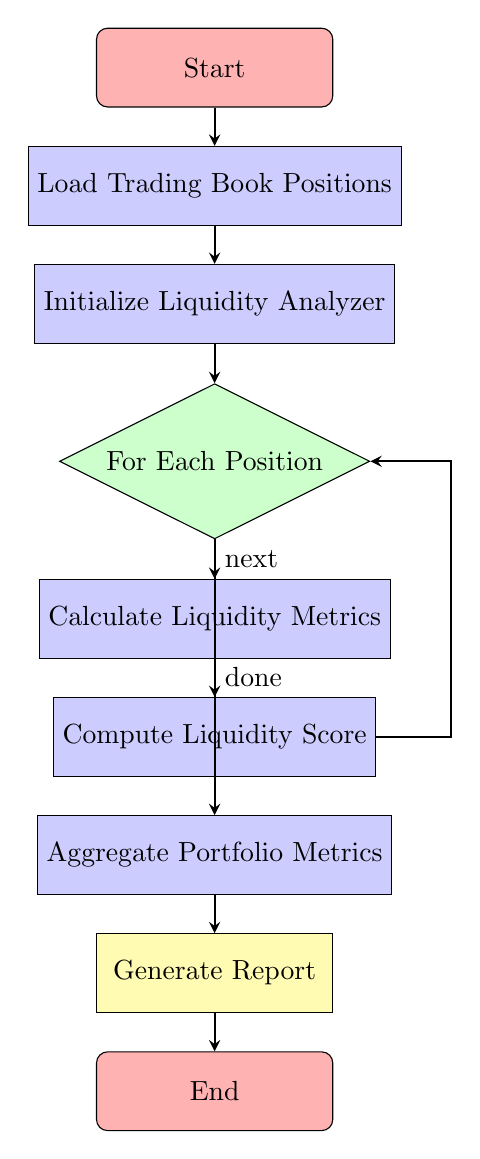
\begin{tikzpicture}[
    node distance=1.5cm,
    startstop/.style={rectangle, rounded corners, minimum width=3cm, minimum height=1cm, text centered, draw=black, fill=red!30},
    process/.style={rectangle, minimum width=3cm, minimum height=1cm, text centered, draw=black, fill=blue!20},
    decision/.style={diamond, minimum width=3cm, minimum height=1cm, text centered, draw=black, fill=green!20, aspect=2},
    output/.style={rectangle, minimum width=3cm, minimum height=1cm, text centered, draw=black, fill=yellow!30},
    arrow/.style={thick,->,>=stealth}
]

\node (start) [startstop] {Start};
\node (input) [process, below of=start] {Load Trading Book Positions};
\node (init) [process, below of=input] {Initialize Liquidity Analyzer};
\node (loop) [decision, below of=init, yshift=-0.5cm] {For Each Position};
\node (calc) [process, below of=loop, yshift=-0.5cm] {Calculate Liquidity Metrics};
\node (score) [process, below of=calc] {Compute Liquidity Score};
\node (agg) [process, below of=score] {Aggregate Portfolio Metrics};
\node (report) [output, below of=agg] {Generate Report};
\node (end) [startstop, below of=report] {End};

\draw [arrow] (start) -- (input);
\draw [arrow] (input) -- (init);
\draw [arrow] (init) -- (loop);
\draw [arrow] (loop) -- node[anchor=west] {next} (calc);
\draw [arrow] (calc) -- (score);
\draw [arrow] (score) -| ++(3,0) |- (loop);
\draw [arrow] (loop) -- node[anchor=west] {done} (agg);
\draw [arrow] (agg) -- (report);
\draw [arrow] (report) -- (end);

\end{tikzpicture}
\caption{High-Level Liquidity Analysis Flow}
\end{figure}

\subsection{Position-Level Metric Calculation}

\begin{figure}[H]
\centering
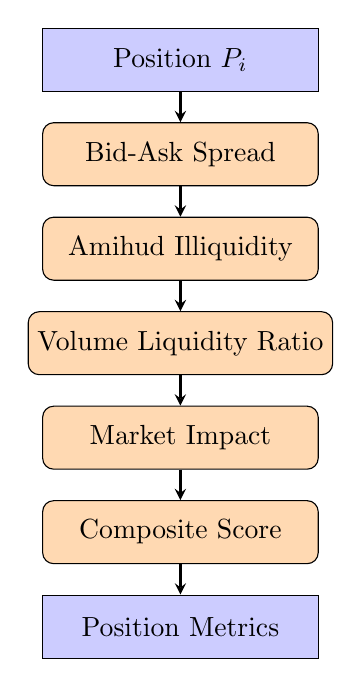
\begin{tikzpicture}[
    node distance=1.2cm,
    process/.style={rectangle, minimum width=3.5cm, minimum height=0.8cm, text centered, draw=black, fill=blue!20},
    metric/.style={rectangle, rounded corners, minimum width=3.5cm, minimum height=0.8cm, text centered, draw=black, fill=orange!30},
    arrow/.style={thick,->,>=stealth}
]

\node (pos) [process] {Position $P_i$};
\node (spread) [metric, below of=pos] {Bid-Ask Spread};
\node (amihud) [metric, below of=spread] {Amihud Illiquidity};
\node (volume) [metric, below of=amihud] {Volume Liquidity Ratio};
\node (impact) [metric, below of=volume] {Market Impact};
\node (score) [metric, below of=impact] {Composite Score};
\node (output) [process, below of=score] {Position Metrics};

\draw [arrow] (pos) -- (spread);
\draw [arrow] (spread) -- (amihud);
\draw [arrow] (amihud) -- (volume);
\draw [arrow] (volume) -- (impact);
\draw [arrow] (impact) -- (score);
\draw [arrow] (score) -- (output);

\end{tikzpicture}
\caption{Position-Level Calculation Sequence}
\end{figure}

\subsection{Market Impact Calculation Flow}

\begin{figure}[H]
\centering
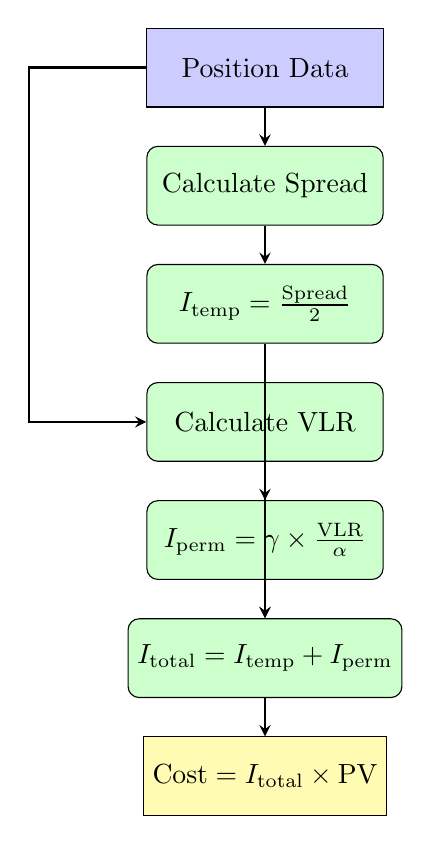
\begin{tikzpicture}[
    node distance=1.5cm,
    process/.style={rectangle, minimum width=3cm, minimum height=1cm, text centered, draw=black, fill=blue!20},
    calc/.style={rectangle, rounded corners, minimum width=3cm, minimum height=1cm, text centered, draw=black, fill=green!20},
    output/.style={rectangle, minimum width=3cm, minimum height=1cm, text centered, draw=black, fill=yellow!30},
    arrow/.style={thick,->,>=stealth}
]

\node (input) [process] {Position Data};
\node (spread) [calc, below of=input] {Calculate Spread};
\node (temp) [calc, below of=spread] {$I_{\text{temp}} = \frac{\text{Spread}}{2}$};
\node (vlr) [calc, below of=temp] {Calculate VLR};
\node (perm) [calc, below of=vlr] {$I_{\text{perm}} = \gamma \times \frac{\text{VLR}}{\alpha}$};
\node (total) [calc, below of=perm] {$I_{\text{total}} = I_{\text{temp}} + I_{\text{perm}}$};
\node (cost) [output, below of=total] {$\text{Cost} = I_{\text{total}} \times \text{PV}$};

\draw [arrow] (input) -- (spread);
\draw [arrow] (spread) -- (temp);
\draw [arrow] (input) -| ++(-3,0) |- (vlr);
\draw [arrow] (temp) -- (total);
\draw [arrow] (vlr) -- (perm);
\draw [arrow] (perm) -- (total);
\draw [arrow] (total) -- (cost);

\end{tikzpicture}
\caption{Market Impact Calculation Flow}
\end{figure}

\subsection{Composite Score Computation}

\begin{figure}[H]
\centering
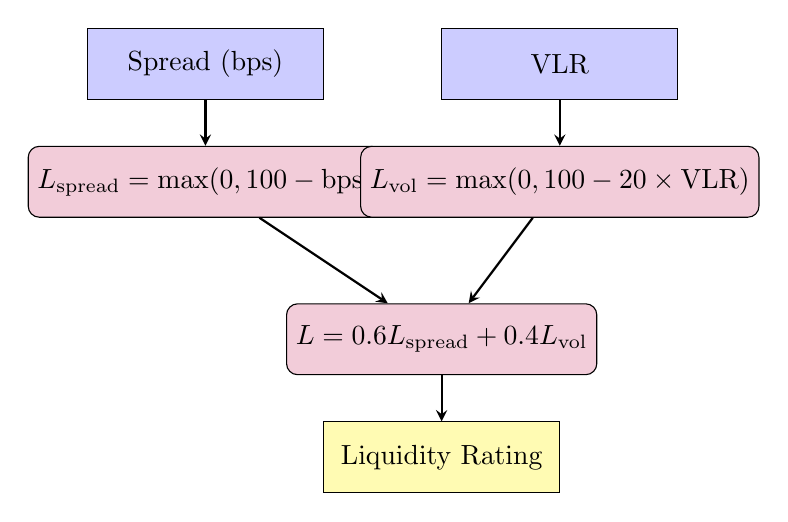
\begin{tikzpicture}[
    node distance=1.5cm,
    process/.style={rectangle, minimum width=3cm, minimum height=0.9cm, text centered, draw=black, fill=blue!20},
    calc/.style={rectangle, rounded corners, minimum width=3.5cm, minimum height=0.9cm, text centered, draw=black, fill=purple!20},
    output/.style={rectangle, minimum width=3cm, minimum height=0.9cm, text centered, draw=black, fill=yellow!30},
    arrow/.style={thick,->,>=stealth}
]

\node (spread_bps) [process] {Spread (bps)};
\node (spread_score) [calc, below of=spread_bps] {$L_{\text{spread}} = \max(0, 100 - \text{bps})$};
\node (vlr) [process, right of=spread_bps, xshift=3cm] {VLR};
\node (vol_score) [calc, below of=vlr] {$L_{\text{vol}} = \max(0, 100 - 20 \times \text{VLR})$};
\node (weighted) [calc, below of=spread_score, xshift=3cm, yshift=-0.5cm] {$L = 0.6 L_{\text{spread}} + 0.4 L_{\text{vol}}$};
\node (rating) [output, below of=weighted] {Liquidity Rating};

\draw [arrow] (spread_bps) -- (spread_score);
\draw [arrow] (vlr) -- (vol_score);
\draw [arrow] (spread_score) -- (weighted);
\draw [arrow] (vol_score) -- (weighted);
\draw [arrow] (weighted) -- (rating);

\end{tikzpicture}
\caption{Composite Liquidity Score Calculation}
\end{figure}

\section{Implementation Algorithm}

\begin{algorithm}
\caption{Trading Book Liquidity Analysis}
\begin{algorithmic}[1]
\Require Trading book $\mathcal{P} = \{P_1, P_2, \ldots, P_N\}$
\Ensure Liquidity metrics for each position and portfolio aggregates

\State Initialize empty results list $\mathcal{R}$

\For{each position $P_i$ in $\mathcal{P}$}
    \State $M_i \gets (B_i + A_i) / 2$ \Comment{Mid-price}
    \State $\text{PV}_i \gets |Q_i| \times M_i$ \Comment{Position value}

    \State \textbf{Calculate spread metrics:}
    \State $\text{Spread}_{\text{abs}} \gets A_i - B_i$
    \State $\text{Spread}_{\text{rel}} \gets \text{Spread}_{\text{abs}} / M_i$
    \State $\text{Spread}_{\text{bps}} \gets \text{Spread}_{\text{rel}} \times 10000$

    \State \textbf{Calculate Amihud illiquidity:}
    \State $\text{ILLIQ}_i \gets |R_i| / (V_i \times M_i)$

    \State \textbf{Calculate volume ratio:}
    \State $\text{VLR}_i \gets |Q_i| / V_i$
    \State $T_{\text{liq}} \gets \text{VLR}_i / \alpha$ \Comment{Time to liquidate}

    \State \textbf{Calculate market impact:}
    \State $I_{\text{temp}} \gets \text{Spread}_{\text{rel}} / 2$
    \State $I_{\text{perm}} \gets \gamma \times T_{\text{liq}}$
    \State $I_{\text{total}} \gets I_{\text{temp}} + I_{\text{perm}}$
    \State $\text{Cost}_i \gets I_{\text{total}} \times \text{PV}_i$

    \State \textbf{Calculate liquidity score:}
    \State $L_{\text{spread}} \gets \max(0, 100 - \text{Spread}_{\text{bps}})$
    \State $L_{\text{vol}} \gets \max(0, 100 - 20 \times \text{VLR}_i)$
    \State $L_i \gets 0.6 \times L_{\text{spread}} + 0.4 \times L_{\text{vol}}$
    \State $\text{Rating}_i \gets \text{ClassifyLiquidity}(L_i)$

    \State Add all metrics to $\mathcal{R}$
\EndFor

\State \textbf{Calculate portfolio aggregates:}
\State $\text{PV}_{\mathcal{P}} \gets \sum_{i=1}^{N} \text{PV}_i$
\State $\overline{\text{Spread}} \gets \sum_{i=1}^{N} (\text{Spread}_{\text{bps},i} \times \text{PV}_i) / \text{PV}_{\mathcal{P}}$
\State $\text{Cost}_{\mathcal{P}} \gets \sum_{i=1}^{N} \text{Cost}_i$
\State $\text{LCR}_{\mathcal{P}} \gets 100 \times \text{Cost}_{\mathcal{P}} / \text{PV}_{\mathcal{P}}$

\Return $\mathcal{R}$, portfolio aggregates
\end{algorithmic}
\end{algorithm}

\section{Practical Example}

Consider a trading book with four positions:

\begin{table}[H]
\centering
\caption{Example Trading Book}
\begin{tabular}{@{}lrrrrrr@{}}
\toprule
Symbol & Quantity & Price & Bid & Ask & Daily Vol & Position Value \\
\midrule
AAPL & 10,000 & 180.50 & 180.48 & 180.52 & 50,000,000 & \$1,805,000 \\
TSLA & 5,000 & 242.80 & 242.70 & 242.90 & 100,000,000 & \$1,214,000 \\
SMALL & 50,000 & 15.25 & 15.10 & 15.40 & 100,000 & \$762,500 \\
MICRO & 100,000 & 2.50 & 2.40 & 2.60 & 50,000 & \$250,000 \\
\bottomrule
\end{tabular}
\end{table}

\subsection{AAPL Analysis}

\textbf{Spread Metrics:}
\begin{align*}
\text{Spread}_{\text{abs}} &= 180.52 - 180.48 = 0.04 \\
\text{Spread}_{\text{rel}} &= \frac{0.04}{180.50} = 0.0221\% \\
\text{Spread}_{\text{bps}} &= 2.21
\end{align*}

\textbf{Volume Ratio:}
\begin{align*}
\text{VLR} &= \frac{10,000}{50,000,000} = 0.0002 \\
T_{\text{liq}} &= \frac{0.0002}{0.10} = 0.002 \text{ days} < 1 \text{ hour}
\end{align*}

\textbf{Market Impact:}
\begin{align*}
I_{\text{temp}} &= \frac{0.0221\%}{2} = 0.011\% \\
I_{\text{perm}} &= 0.1\% \times 0.002 = 0.0002\% \\
I_{\text{total}} &= 0.0112\% \\
\text{Cost} &= 0.0112\% \times \$1,805,000 = \$202
\end{align*}

\textbf{Liquidity Score:}
\begin{align*}
L_{\text{spread}} &= \max(0, 100 - 2.21) = 97.79 \\
L_{\text{vol}} &= \max(0, 100 - 20 \times 0.0002) = 99.996 \\
L &= 0.6 \times 97.79 + 0.4 \times 99.996 = 98.67 \\
\text{Rating} &= \text{Highly Liquid}
\end{align*}

\subsection{MICRO Analysis (Illiquid Position)}

\textbf{Spread Metrics:}
\begin{align*}
\text{Spread}_{\text{abs}} &= 2.60 - 2.40 = 0.20 \\
\text{Spread}_{\text{rel}} &= \frac{0.20}{2.50} = 8.0\% \\
\text{Spread}_{\text{bps}} &= 800
\end{align*}

\textbf{Volume Ratio:}
\begin{align*}
\text{VLR} &= \frac{100,000}{50,000} = 2.0 \\
T_{\text{liq}} &= \frac{2.0}{0.10} = 20 \text{ days}
\end{align*}

\textbf{Market Impact:}
\begin{align*}
I_{\text{temp}} &= \frac{8.0\%}{2} = 4.0\% \\
I_{\text{perm}} &= 0.1\% \times 20 = 2.0\% \\
I_{\text{total}} &= 6.0\% \\
\text{Cost} &= 6.0\% \times \$250,000 = \$15,000
\end{align*}

\textbf{Liquidity Score:}
\begin{align*}
L_{\text{spread}} &= \max(0, 100 - 800) = 0 \\
L_{\text{vol}} &= \max(0, 100 - 20 \times 2.0) = 60 \\
L &= 0.6 \times 0 + 0.4 \times 60 = 24 \\
\text{Rating} &= \text{Illiquid}
\end{align*}

\section{Interpretation and Usage}

\subsection{Position-Level Decisions}

\begin{itemize}
    \item \textbf{$L \geq 80$:} Can be liquidated quickly with minimal market impact. Suitable for high-turnover strategies.
    \item \textbf{$60 \leq L < 80$:} Normal liquidity. Standard execution algorithms appropriate.
    \item \textbf{$40 \leq L < 60$:} Requires careful execution over multiple days. Consider VWAP/TWAP algorithms.
    \item \textbf{$20 \leq L < 40$:} Significant liquidity constraints. May require weeks to exit. Consider position limits.
    \item \textbf{$L < 20$:} Highly illiquid. Requires specialized broker relationships or block trading.
\end{itemize}

\subsection{Portfolio-Level Risk Management}

The portfolio liquidity cost ratio (LCR) provides a single metric for overall book liquidity:

\begin{equation}
\text{Risk}(\text{LCR}_{\mathcal{P}}) = \begin{cases}
\text{Low} & \text{if LCR} < 0.5\% \\
\text{Moderate} & \text{if } 0.5\% \leq \text{LCR} < 2.0\% \\
\text{High} & \text{if } 2.0\% \leq \text{LCR} < 5.0\% \\
\text{Extreme} & \text{if LCR} \geq 5.0\%
\end{cases}
\end{equation}

\subsection{Regulatory Applications}

\textbf{Basel III Liquidity Coverage Ratio (LCR):}
Positions with high liquidation costs and long liquidation times should receive appropriate haircuts when calculating high-quality liquid assets (HQLA).

\textbf{SEC Rule 22e-4 (Mutual Fund Liquidity):}
US mutual funds must classify positions into liquidity buckets. This framework maps directly:
\begin{itemize}
    \item Highly Liquid: $T_{\text{liq}} \leq 3$ days
    \item Moderately Liquid: $3 < T_{\text{liq}} \leq 7$ days
    \item Less Liquid: $7 < T_{\text{liq}} \leq 15$ days
    \item Illiquid: $T_{\text{liq}} > 15$ days
\end{itemize}

\section{Model Limitations and Extensions}

\subsection{Current Limitations}

\begin{enumerate}
    \item \textbf{Static Analysis:} Does not account for time-varying liquidity (intraday patterns, market stress)
    \item \textbf{Simplified Impact Model:} Real market impact exhibits non-linear behavior
    \item \textbf{No Correlation:} Ignores correlation between positions during fire-sale scenarios
    \item \textbf{Single Market:} Does not account for multi-venue or international execution
\end{enumerate}

\subsection{Potential Extensions}

\subsubsection{Conditional Liquidity}

Incorporate regime-switching models:

\begin{equation}
\text{Spread}_i(t) = \text{Spread}_{\text{normal},i} \times \left(1 + \lambda_t \right)
\end{equation}

where $\lambda_t$ represents a market stress factor.

\subsubsection{Optimal Execution}

Integrate with Almgren-Chriss optimal execution framework:

\begin{equation}
\text{Cost}_{\text{opt}} = \frac{\sigma^2 \tau}{2\eta} + \frac{\eta Q^2}{2\tau}
\end{equation}

where $\tau$ is execution time, $\eta$ is temporary impact parameter, and $\sigma$ is volatility.

\subsubsection{Network Effects}

Model portfolio-wide liquidation using fire-sale externalities:

\begin{equation}
\text{Impact}_{\text{portfolio}} > \sum_{i=1}^{N} \text{Impact}_i
\end{equation}

\section{Conclusion}

This framework provides a comprehensive, mathematically rigorous approach to measuring trading book liquidity. By combining multiple established metrics into a unified system, it enables quantitative risk management, portfolio optimization under liquidity constraints, and regulatory compliance.

The composite liquidity score offers a simple summary metric while preserving the detailed multi-dimensional analysis needed for sophisticated applications. Implementation in Python enables rapid analysis of large trading books and integration into existing risk management systems.

\section{References}

\begin{enumerate}
    \item Amihud, Y. (2002). Illiquidity and stock returns: cross-section and time-series effects. \textit{Journal of Financial Markets}, 5(1), 31-56.

    \item Almgren, R., \& Chriss, N. (2001). Optimal execution of portfolio transactions. \textit{Journal of Risk}, 3, 5-40.

    \item Kyle, A. S. (1985). Continuous auctions and insider trading. \textit{Econometrica}, 53(6), 1315-1335.

    \item Hasbrouck, J. (2009). Trading costs and returns for US equities: Estimating effective costs from daily data. \textit{The Journal of Finance}, 64(3), 1445-1477.

    \item Basel Committee on Banking Supervision (2013). Basel III: The Liquidity Coverage Ratio and liquidity risk monitoring tools.

    \item SEC (2016). Investment Company Liquidity Risk Management Programs; Commission Guidance for In-Kind ETFs. Rule 22e-4.
\end{enumerate}

\end{document}
